% ---------------------------------------------------------------------
% Podstawowe ustawienia i pakiety
% ---------------------------------------------------------------------
\RequirePackage[l2tabu, orthodox]{nag}  % Wykrywa przestarzałe i niewłaściwe
% sposoby używania LaTeXa. Więcej jest w l2tabu English version.
\documentclass[a4paper,11pt]{article}
% {rozmiar papieru, rozmiar fontu}[klasa dokumentu]
\usepackage[MeX]{polski}  % Polonizacja LaTeXa, bez niej będzie pracował
% w języku angielskim.
\usepackage[utf8]{inputenc} % Włączenie kodowania UTF-8, co daje dostęp
% do polskich znaków.
\usepackage{lmodern}  % Wprowadza fonty Latin Modern.
\usepackage[T1]{fontenc}  % Potrzebne do używania fontów Latin Modern.



% ------------------------------
% Podstawowe pakiety (niezwiązane z ustawieniami języka)
% ------------------------------
\usepackage{microtype}  % Twierdzi, że poprawi rozmiar odstępów w tekście.
\usepackage{graphicx}  % Wprowadza bardzo potrzebne komendy do wstawiania
% grafiki.
% \usepackage{verbatim}  % Poprawia otoczenie VERBATIME.
% \usepackage{textcomp}  % Dodaje takie symbole jak stopnie Celsiusa,
% wprowadzane bezpośrednio w tekście.
\usepackage{vmargin}  % Pozwala na prostą kontrolę rozmiaru marginesów,
% za pomocą komend poniżej. Rozmiar odstępów jest mierzony w calach.
% ------------------------------
% MARGINS
% ------------------------------
\setmarginsrb
{ 0.7in} % left margin
{ 0.6in} % top margin
{ 0.7in} % right margin
{ 0.8in} % bottom margin
{  20pt} % head height
{0.25in} % head sep
{   9pt} % foot height
{ 0.3in} % foot sep



% ------------------------------
% Często przydatne pakiety
% ------------------------------
% \usepackage{csquotes}  % Pozwala w prosty sposób wstawiać cytaty do tekstu.




% ------------------------------
% Pakiety do tekstów z nauk przyrodniczych
% ------------------------------
\let\lll\undefined  % Amsmath gryzie się z pakietami do języka
% polskiego, bo oba definiują komendę \lll. Aby rozwiązać ten problem
% oddefiniowuję tę komendę, ale może tym samym pozbywam się dużego Ł.
\usepackage[intlimits]{amsmath}  % Podstawowe wsparcie od American
% Mathematical Society (w skrócie AMS)
\usepackage{amsfonts, amssymb, amscd, amsthm}  % Dalsze wsparcie od AMS
% \usepackage{siunitx}  % Do prostszego pisania jednostek fizycznych
\usepackage{upgreek}  % Ładniejsze greckie litery
% Przykładowa składnia: pi = \uppi
% \usepackage{slashed}  % Pozwala w prosty sposób pisać slash Feynmana.
\usepackage{calrsfs}  % Zmienia czcionkę kaligraficzną w \mathcal
% na ładniejszą. Może w innych miejscach robi to samo, ale o tym nic
% nie wiem.





% ------------------------------
% Paczki, biblioteki i ich ustawienia dla tego pliku
% ------------------------------
\usepackage{tikz}  % Wspaniały pakiet PGF/TikZ

% \listfiles







% ------------------------------
% Pakiet „hyperref”
% Polecano by umieszczać go na końcu preambuły
% ------------------------------
\usepackage{hyperref}  % Pozwala tworzyć hiperlinki i zamienia odwołania
% do bibliografii na hiperlinki










% ---------------------------------------------------------------------
% Tytuł, autor, data
\title{Ti\textit{k}Z \& PGF \\
  \href{http://piotrkosoft.net/pub/mirrors/CTAN/graphics/pgf/base/doc/pgfmanual.pdf}{Manual for version 3.1.9a} \\
  2~A~Picture for Karl's Students}
% \href{http://piotrkosoft.net/pub/mirrors/CTAN/graphics/pgf/base/doc/pgfmanual.pdf}{Ti\textit{k}Z \& PGF Manual, v. 3.1.8b} \\
%   14~Syntax for Path Specifications, part~I}

\author{}


% \date{}
% ---------------------------------------------------------------------










% ####################################################################
\begin{document}
% ####################################################################





% ######################################
\maketitle % Tytuł całego tekstu
% ######################################





% ######################################
\section{Part I. Tutorials and Guidelines}

\vspace{2em}

% ######################################


\tikz \draw[thick,rounded corners=8pt] (0,0) -- (0,2) -- (1,3.25) --
(2,2) -- (2,0) -- (0,2) -- (2,2) -- (0,0) -- (2,0);










% ######################################
\newpage

\section{2~Tutorial: A~Picture for Karl's Students}

\vspace{2em}

% ######################################





\tikz \draw (-1.5,0) -- (1.5,0) -- (0,-1.5) -- (0,1.5); \hspace{2em}
Abc \tikz{\draw (0,0) -- (1.5,0)} def. \hspace{2em}
Abc \tikz \draw (0,0) -- (1.5,0); def.

\vspace{2em}



Abc \tikz \draw (0,0) circle [radius=10pt]; def. \hspace{2em}
Abc \tikz \draw (0,0) ellipse [x radius=20pt, y radius=10pt]; def.
\hspace{2em}
Abc \tikz \draw[rotate=30] (0,0) ellipse [x radius=6pt, y radius=3pt]; def.

\vspace{2em}



Abc \tikz \draw[step=2pt] (0,0) grid (10pt,10pt); def.

\vspace{2em}



Abc \tikz \draw[step=0.5] (0,0) grid (2,2); def.

\vspace{2em}



Coś tu jest nie tak.

\tikzset{help lines test/.style=very thin}


Abc 1 \tikz \draw[help lines,step=0.5] (0,0) grid (2,2); def. \hspace{2em}
Abc 2 \tikz \draw[help lines,very thin,step=0.5] (0,0) grid (2,2); def.
\hspace{2em}
Abc 3 \tikz \draw[help lines test,step=0.5] (0,0) grid (2,2); def.

\vspace{2em}



Abc 4 \tikz \draw[very thin,step=0.5] (0,0) grid (2,2); def. \hspace{2em}
Abc 5 \tikz \draw[very thin,help lines,step=0.5] (0,0) grid (2,2); def.





% ##################
\begin{figure}[ht]

  \centering

  \begin{tikzpicture}

    \draw (-1.5,0) -- (1.5,0);

    \draw (0,-1.5) -- (0,1.5);

  \end{tikzpicture}

  \caption{Ti\textit{k}Z \& PGF Manula. A~Picture for Karl's Students,~1}

\end{figure}
% ##################





% ##################
\begin{figure}[ht]

  \centering

  \begin{tikzpicture}

    \draw (-1.5,0) -- (1.5,0) -- (0,-1.5) -- (0,1.5);

  \end{tikzpicture}

  \caption{Ti\textit{k}Z \& PGF Manula. A~Picture for Karl's Students,~2}

\end{figure}
% ##################





% ##################
\begin{figure}[ht]

  \centering

  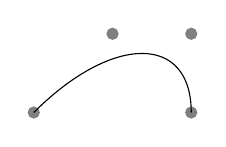
\begin{tikzpicture}

    \filldraw[gray] (0,0) circle [radius=2pt]
    (1,1) circle [radius=2pt]
    (2,1) circle [radius=2pt]
    (2,0) circle [radius=2pt];

    \draw (0,0) .. controls (1,1) and (2,1) .. (2,0);

  \end{tikzpicture}

  \caption{Ti\textit{k}Z \& PGF Manula. A~Picture for Karl's Students,~3}

\end{figure}
% ##################





% ##################
\begin{figure}[ht]

  \centering

  \begin{tikzpicture}

    \draw (-1.5,0) -- (1.5,0);

    \draw (0,-1.5) -- (0,1.5);

    \draw (-1,0) .. controls (-1,0.555) and (-0.555,1) .. (0,1)
    .. controls (0.555,1) and (1,0.555) .. (1,0);

  \end{tikzpicture}

  \caption{Ti\textit{k}Z \& PGF Manula. A~Picture for Karl's Students,~4}

\end{figure}
% ##################





% ##################
\begin{figure}[ht]

  \centering

  \begin{tikzpicture}

    \draw (-1.5,0) -- (1.5,0);

    \draw (0,-1.5) -- (0,1.5);

    \draw (0,0) circle [radius=1cm];

  \end{tikzpicture}

  \caption{Ti\textit{k}Z \& PGF Manula. A~Picture for Karl's Students,~5}

\end{figure}
% ##################





% ##################
\begin{figure}[ht]

  \centering

  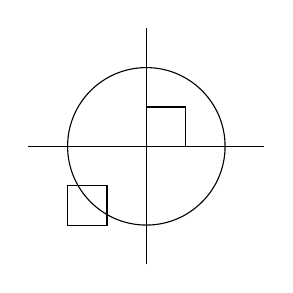
\begin{tikzpicture}

    \draw (-1.5,0) -- (1.5,0);

    \draw (0,-1.5) -- (0,1.5);

    \draw (0,0) circle [radius=1cm];

    \draw (0,0) rectangle (0.5,0.5);

    \draw (-0.5,-0.5) rectangle (-1,-1);

  \end{tikzpicture}

  \caption{Ti\textit{k}Z \& PGF Manula. A~Picture for Karl's Students,~6}

\end{figure}
% ##################





% ##################
\begin{figure}[ht]

  \centering

  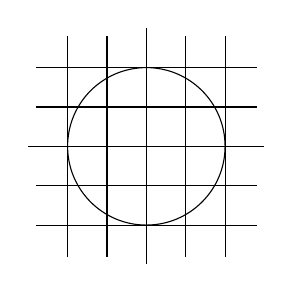
\begin{tikzpicture}

    \draw (-1.5,0) -- (1.5,0);

    \draw (0,-1.5) -- (0,1.5);

    \draw (0,0) circle [radius=1cm];

    \draw[step=0.5cm] (-1.4,-1.4) grid (1.4,1.4);

  \end{tikzpicture}

  \caption{Ti\textit{k}Z \& PGF Manula. A~Picture for Karl's Students,~7}

\end{figure}
% ##################





% ##################
\begin{figure}[ht]

  \centering

  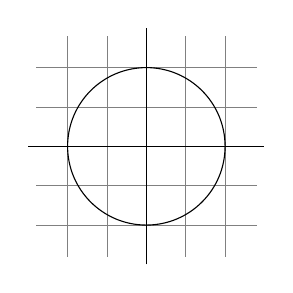
\begin{tikzpicture}

    \draw[step=0.5cm,gray,very thin] (-1.4,-1.4) grid (1.4,1.4);

    \draw (-1.5,0) -- (1.5,0);

    \draw (0,-1.5) -- (0,1.5);

    \draw (0,0) circle [radius=1cm];

  \end{tikzpicture}

  \caption{Ti\textit{k}Z \& PGF Manula. A~Picture for Karl's Students,~8}

\end{figure}
% ##################





% ##################
\begin{figure}[ht]
  \centering

  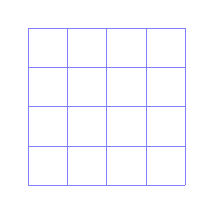
\begin{tikzpicture}[help lines/.style={color=blue!50,very thin}]

    \draw[help lines,step=0.5] (0,0) grid (2,2);

  \end{tikzpicture}

  \caption{Ti\textit{k}Z \& PGF Manula. A~Picture for Karl's Students,~9}

\end{figure}
% ##################





\tikzset{Karl's grid/.style={help lines,color=blue!50}}

% ##################
\begin{figure}[ht]

  \centering

  \begin{tikzpicture}

    \draw[Karl's grid,step=0.5] (0,0) grid (2,2);

  \end{tikzpicture}

  \caption{Ti\textit{k}Z \& PGF Manula. A~Picture for Karl's Students,~10}

\end{figure}
% ##################





% ##################
\begin{figure}[ht]
  \centering

  \begin{tikzpicture}
    [Karl's grid one/.style ={help lines,color=#1!50},
    Karl's grid one/.default=blue]


    \draw[Karl's grid one] (0,0) grid (1.5,2);

    \draw[Karl's grid one=red] (2,0) grid (3.5,2);

  \end{tikzpicture}

  \caption{Ti\textit{k}Z \& PGF Manula. A~Picture for Karl's Students,~11}

\end{figure}
% ##################





% ##################
\begin{figure}[ht]

  \centering

  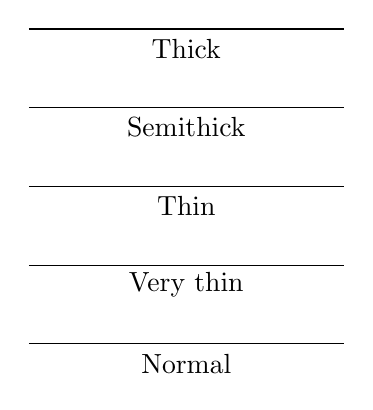
\begin{tikzpicture}

    \draw (0,0) -- (4,0);

    \node at (2,-0.25) {Normal};


    \draw[very thin] (0,1) -- (4,1);

    \node at (2,0.75) {Very thin};


    \draw[thin] (0,2) -- (4,2);

    \node at (2,1.75) {Thin};


    \draw[semithick] (0,3) -- (4,3);

    \node at (2,2.75) {Semithick};


    \draw[thick] (0,4) -- (4,4);

    \node at (2,3.75) {Thick};

  \end{tikzpicture}

  \caption{Ti\textit{k}Z \& PGF Manula. A~Picture for Karl's Students,~12}

\end{figure}
% ##################





% ##################
\begin{figure}[ht]

  \centering

  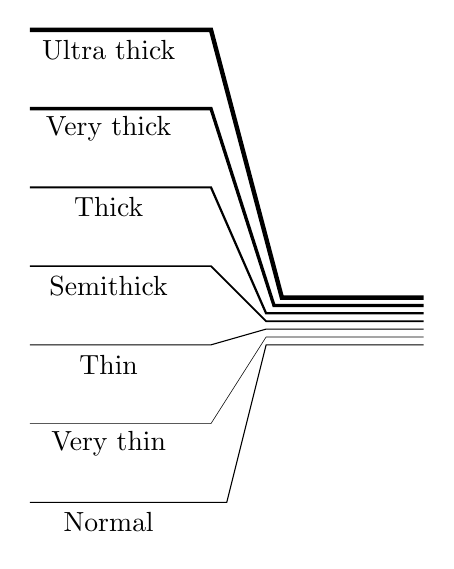
\begin{tikzpicture}

    \draw (-3,-3) -- (-0.5,-3) -- (0,-1) -- (2,-1);

    \node at (-2,-3.25) {Normal};


    \draw[very thin] (-3,-2) -- (-0.7,-2) -- (0,-0.9) -- (2,-0.9);

    \node at (-2,-2.25) {Very thin};


    \draw[thin] (-3,-1) -- (-0.7,-1) -- (0,-0.8) -- (2,-0.8);

    \node at (-2,-1.25) {Thin};


    \draw[semithick] (-3,0) -- (-0.7,0) -- (0,-0.7) -- (2,-0.7);

    \node at (-2,-0.25) {Semithick};


    \draw[thick] (-3,1) -- (-0.7,1) -- (0,-0.6) -- (2,-0.6);

    \node at (-2,0.75) {Thick};


    \draw[very thick] (-3,2) -- (-0.7,2) -- (0.1,-0.5) -- (2,-0.5);

    \node at (-2,1.75) {Very thick};


    \draw[ultra thick] (-3,3) -- (-0.7,3) -- (0.2,-0.4) -- (2,-0.4);

    \node at (-2,2.75) {Ultra thick};

  \end{tikzpicture}

  \caption{Ti\textit{k}Z \& PGF Manula. A~Picture for Karl's Students,~13}

\end{figure}
% ##################





% ##################
\begin{figure}[ht]

  \centering

  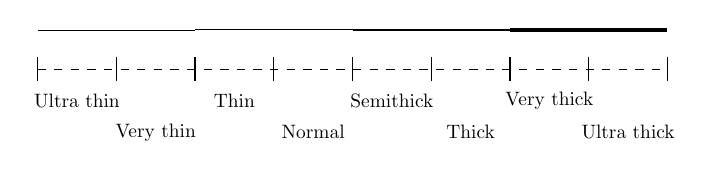
\begin{tikzpicture}

    \draw[dashed] (0,-0.5) -- (8,-0.5);

    \draw (0,-0.65) -- (0,-0.35);

    \draw (1,-0.65) -- (1,-0.35);

    \draw (2,-0.65) -- (2,-0.35);

    \draw (3,-0.65) -- (3,-0.35);

    \draw (4,-0.65) -- (4,-0.35);

    \draw (5,-0.65) -- (5,-0.35);

    \draw (6,-0.65) -- (6,-0.35);

    \draw (7,-0.65) -- (7,-0.35);

    \draw (8,-0.65) -- (8,-0.35);


    \node[scale=0.7] at (0.5,-0.9) {Ultra thin};

    \node[scale=0.7] at (1.5,-1.3) {Very thin};

    \node[scale=0.7] at (2.5,-0.9) {Thin};

    \node[scale=0.7] at (3.5,-1.3) {Normal};

    \node[scale=0.7] at (4.5,-0.9) {Semithick};

    \node[scale=0.7] at (5.5,-1.3) {Thick};

    \node[scale=0.7] at (6.5,-0.9) {Very thick};

    \node[scale=0.7] at (7.5,-1.3) {Ultra thick};



    \draw[ultra thin] (0,0) -- (1,0);

    \draw[very thin] (1,0) -- (2,0);

    \draw[thin] (2,0) -- (3,0);

    \draw (3,0) -- (4,0);

    \draw[semithick] (4,0) -- (5,0);

    \draw[thick] (5,0) -- (6,0);

    \draw[very thick] (6,0) -- (7,0);

    \draw[ultra thick] (7,0) -- (8,0);

  \end{tikzpicture}

  \caption{Ti\textit{k}Z \& PGF Manula. A~Picture for Karl's Students,~14}

\end{figure}
% ##################





% ##################
\begin{figure}[ht]

  \centering

  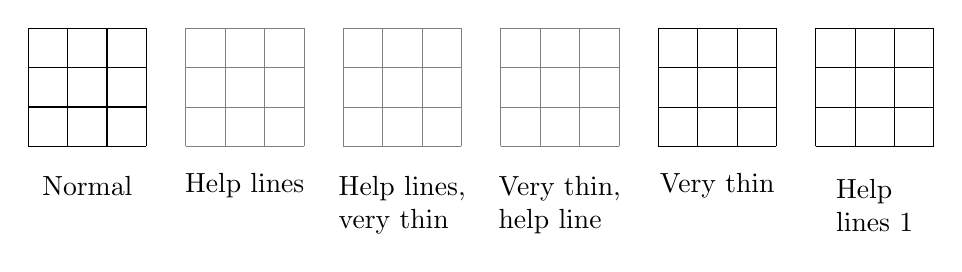
\begin{tikzpicture}[help lines 1/.style={very thin},]

    \draw[step=0.5] (0,0) grid (1.5,1.5);

    \node at (0.75,-0.5) {Normal};



    \begin{scope}[xshift=2cm]

      \draw[help lines,step=0.5] (0,0) grid (1.5,1.5);

      \node at (0.75,-0.5) {Help lines};

    \end{scope}



    \begin{scope}[xshift=4cm]

      \draw[help lines,very thin,step=0.5] (0,0) grid (1.5,1.5);

      \node[align=left] at (0.75,-0.75)
      {Help lines, \\
        very thin};

    \end{scope}



    \begin{scope}[xshift=6cm]

      \draw[very thin,help lines,step=0.5] (0,0) grid (1.5,1.5);

      \node[align=left] at (0.75,-0.75)
      {Very thin, \\
        help line};

    \end{scope}



    \begin{scope}[xshift=8cm]

      \draw[very thin,step=0.5] (0,0) grid (1.5,1.5);

      \node at (0.75,-0.5) {Very thin};

    \end{scope}



    \begin{scope}[xshift=10cm]

      \draw[help lines 1,step=0.5] (0,0) grid (1.5,1.5);

      \node[align=left] at (0.75,-0.75)
      {Help \\
        lines 1};

    \end{scope}

  \end{tikzpicture}

  \caption{Ti\textit{k}Z \& PGF Manula. A~Picture for Karl's Students,~15}

\end{figure}
% ##################





% ##################
\begin{figure}[ht]

  \centering

  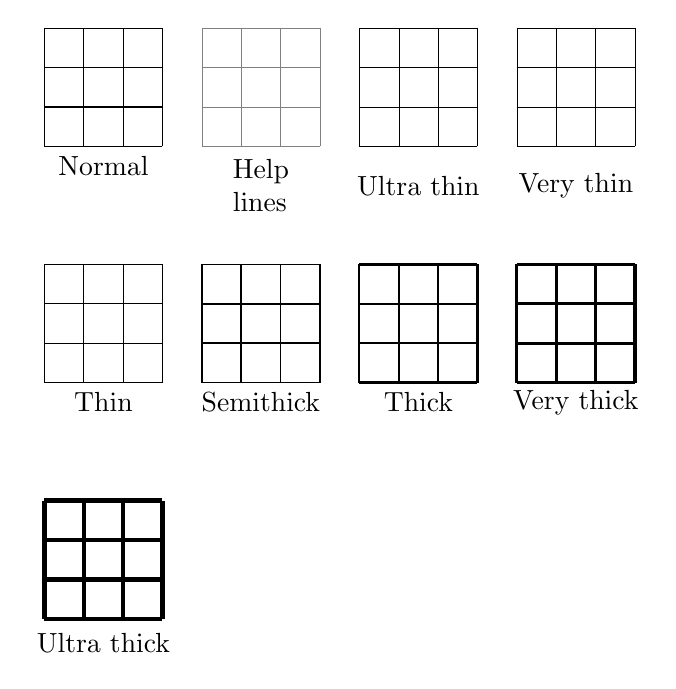
\begin{tikzpicture}

    \draw[step=0.5] (0,0) grid (1.5,1.5);

    \node at (0.75,-0.25) {Normal};



    \begin{scope}[xshift=2cm]

      \draw[help lines,step=0.5] (0,0) grid (1.5,1.5);

      \node[align=left] at (0.75,-0.5)
      {Help \\
        lines};

    \end{scope}



    \begin{scope}[xshift=4cm]

      \draw[ultra thin,step=0.5] (0,0) grid (1.5,1.5);

      \node at (0.75,-0.5) {Ultra thin};

    \end{scope}



    \begin{scope}[xshift=6cm]

      \draw[very thin,step=0.5] (0,0) grid (1.5,1.5);

      \node at (0.75,-0.5) {Very thin};

    \end{scope}





    \begin{scope}[yshift=-3cm]

      \draw[thin,step=0.5] (0,0) grid (1.5,1.5);

      \node at (0.75,-0.25) {Thin};

    \end{scope}



    \begin{scope}[xshift=2cm,yshift=-3cm]

      \draw[semithick,step=0.5] (0,0) grid (1.5,1.5);

      \node at (0.75,-0.25) {Semithick};

    \end{scope}



    \begin{scope}[xshift=4cm,yshift=-3cm]

      \draw[thick,step=0.5] (0,0) grid (1.5,1.5);

      \node at (0.75,-0.25) {Thick};

    \end{scope}



    \begin{scope}[xshift=6cm,yshift=-3cm]

      \draw[very thick,step=0.5] (0,0) grid (1.5,1.5);

      \node at (0.75,-0.25) {Very thick};

    \end{scope}





    \begin{scope}[yshift=-6cm]

      \draw[ultra thick,step=0.5] (0,0) grid (1.5,1.5);

      \node at (0.75,-0.3) {Ultra thick};

    \end{scope}

  \end{tikzpicture}

  \caption{Ti\textit{k}Z \& PGF Manula. A~Picture for Karl's Students,~16}

\end{figure}
% ##################





% ##################
\begin{figure}[ht]

  \centering

  \begin{tikzpicture}






  \end{tikzpicture}

  \caption{Ti\textit{k}Z \& PGF Manula. A~Picture for Karl's Students,~17}

\end{figure}
% ##################





% % ##################
% \begin{figure}[ht]
%   \centering

%   \def\wall{ \fill [fill=black!50] (1,-0.5) rectangle (2,0.5);
%     \pattern [pattern=bricks] (1,-0.5) rectangle (2,0.5);
%     \draw [line width=1pt] (1cm+0.5pt,-0.5) -- ++(0,1);
%   }

%   \begin{tikzpicture}
%     \wall

%     \draw [red!25,line width=1mm] (-1,0) -- (1,0);

%     \draw [red,line width=1mm,-{Stealth[length=1cm,open,blue,quick]}]
%     (-1,-0.5) .. controls (0,-0.5) and (0,0) .. (1,0);
%   \end{tikzpicture}

%   \caption{Ti\emph{k}Z 18.}
% \end{figure}
% % ##################





% % ##################
% \begin{figure}[ht]
%   \centering

%   \def\wall{ \fill [fill=black!50] (1,-0.5) rectangle (2,0.5);
%     \pattern [pattern=bricks] (1,-0.5) rectangle (2,0.5);
%     \draw [line width=1pt] (1cm+0.5pt,-0.5) -- ++(0,1);
%   }

%   \begin{tikzpicture}
%     \wall

%     \draw [red!25,line width=1mm] (-1,0) -- (1,0);

%     \draw [red,line width=1mm,-{[quick,sep]>>>}]
%     (-1,-0.5) .. controls (0,-0.5) and (0,0) .. (1,0);
%   \end{tikzpicture}

%   \caption{Ti\emph{k}Z 19.}
% \end{figure}
% % ##################


Strona 200 bending.


% % ##################
% \begin{figure}[ht]
%   \centering

%   \begin{tikzpicture}

%   \end{tikzpicture}

%   \caption{Ti\emph{k}Z .}
% \end{figure}
% % ##################





% % ##################
% \begin{figure}[ht]
%   \centering

%   \begin{tikzpicture}

%   \end{tikzpicture}

%   \caption{Ti\emph{k}Z .}
% \end{figure}
% % ##################





% % ##################
% \begin{figure}[ht]
%   \centering

%   \begin{tikzpicture}

%   \end{tikzpicture}

%   \caption{Ti\emph{k}Z .}
% \end{figure}
% % ##################





% % ##################
% \begin{figure}[ht]
%   \centering

%   \begin{tikzpicture}

%   \end{tikzpicture}

%   \caption{Ti\emph{k}Z .}
% \end{figure}
% % ##################





% % ##################
% \begin{figure}[ht]
%   \centering

%   \begin{tikzpicture}

%   \end{tikzpicture}

%   \caption{Ti\emph{k}Z .}
% \end{figure}
% % ##################





% % ##################
% \begin{figure}[ht]
%   \centering

%   \begin{tikzpicture}



%   \end{tikzpicture}

%   \caption{Ti\emph{k}Z .}
% \end{figure}
% % ##################





% % ##################
% \begin{figure}[ht]
%   \centering

%   \begin{tikzpicture}



%   \end{tikzpicture}

%   \caption{Ti\emph{k}Z .}
% \end{figure}
% % ##################





% % ##################
% \begin{figure}[ht]
%   \centering

%   \begin{tikzpicture}



%   \end{tikzpicture}

%   \caption{Ti\emph{k}Z .}
% \end{figure}
% % ##################





% % ##################
% \begin{figure}[ht]
%   \centering

%   \begin{tikzpicture}

%   \end{tikzpicture}

%   \caption{Ti\emph{k}Z .}
% \end{figure}
% % ##################





% % ##################
% \begin{figure}[ht]
%   \centering

%   \begin{tikzpicture}


%   \end{tikzpicture}

%   \caption{Ti\emph{k}Z .}
% \end{figure}
% % ##################





% % ##################
% \begin{figure}[ht]
%   \centering

%   \begin{tikzpicture}


%   \end{tikzpicture}

%   \caption{Ti\emph{k}Z .}
% \end{figure}
% % ##################





% % ##################
% \begin{figure}[ht]
%   \centering

%   \begin{tikzpicture}




%   \end{tikzpicture}

%   \caption{Ti\emph{k}Z .}
% \end{figure}
% % ##################





% % ##################
% \begin{figure}[ht]
%   \centering

%   \begin{tikzpicture}




%   \end{tikzpicture}

%   \caption{Ti\emph{k}Z .}
% \end{figure}
% % ##################





% % ##################
% \begin{figure}[ht]
%   \centering

%   \begin{tikzpicture}

%   \end{tikzpicture}

%   \caption{Ti\emph{k}Z .}
% \end{figure}
% % ##################





% % ##################
% \begin{figure}[ht]
%   \centering

%   \begin{tikzpicture}





%   \end{tikzpicture}

%   \caption{Ti\emph{k}Z .}
% \end{figure}
% % ##################





% % ##################
% \begin{figure}[ht]
%   \centering

%   \begin{tikzpicture}





%   \end{tikzpicture}

%   \caption{Ti\emph{k}Z .}
% \end{figure}
% % ##################





% % ##################
% \begin{figure}[ht]
%   \centering

%   \begin{tikzpicture}



%   \end{tikzpicture}

%   \caption{Ti\emph{k}Z .}
% \end{figure}
% % ##################





% % ##################
% \begin{figure}[ht]
%   \centering

%   \begin{tikzpicture}





%   \end{tikzpicture}

%   \caption{Ti\emph{k}Z .}
% \end{figure}
% % ##################





% % ##################
% \begin{figure}[ht]
%   \centering

%   \begin{tikzpicture}





%   \end{tikzpicture}

%   \caption{Ti\emph{k}Z .}
% \end{figure}
% % ##################





% % ##################
% \begin{figure}[ht]
%   \centering

%   \begin{tikzpicture}





%   \end{tikzpicture}

%   \caption{Ti\emph{k}Z .}
% \end{figure}
% % ##################





% % ##################
% \begin{figure}[ht]
%   \centering

%   \begin{tikzpicture}





%   \end{tikzpicture}

%   \caption{Ti\emph{k}Z .}
% \end{figure}
% % ##################





% % ##################
% \begin{figure}[ht]
%   \centering

%   \begin{tikzpicture}
%     \draw[arrows = {-Stealth[]}] (0,1) -- (1,1);

%     \draw[arrows = {-Stealth[scale width=1.5]}] (0,0.5) -- (1,0.5);

%     \draw[arrows = {-Stealth[scale width=2]}] (0,0) -- (1,0);
%   \end{tikzpicture}

%   \caption{Ti\emph{k}Z 28.}
% \end{figure}
% % ##################





% % ##################
% \begin{figure}[ht]
%   \centering

%   \begin{tikzpicture}[ultra thick]
%     \draw[arrows = {-Hooks[]}] (0,1) -- (1,1);

%     \draw[arrows = {-Hooks[arc=90]}] (0,0.5) -- (1,0.5);

%     \draw[arrows = {-Hooks[arc=270]}] (0,0) -- (1,0);
%   \end{tikzpicture}

%   \caption{Ti\emph{k}Z 29.}
% \end{figure}
% % ##################





% % ##################
% \begin{figure}[ht]
%   \centering

%   \begin{tikzpicture}
%     \draw[arrows = {->[]}] (0,1) -- (1,1);

%     \draw[arrows = {->[slant=0.5]}] (0,0.5) -- (1,0.5);

%     \draw[arrows = {->[slant=1]}] (0,0) -- (1,0);
%   \end{tikzpicture}

%   \caption{Ti\emph{k}Z 30.}
% \end{figure}
% % ##################





% % ##################
% \begin{figure}[ht]
%   \centering

%   \begin{tikzpicture}[>={[slant=0.3] To[] To[]}]
%     \graph [math nodes] { A -> B -> C };
%   \end{tikzpicture}

%   \caption{Ti\emph{k}Z 31.}
% \end{figure}
% % ##################





% % ##################
% \begin{figure}[ht]
%   \centering

%   \begin{tikzpicture}
%     \draw[ultra thick, arrows = {-Stealth[reversed]}] (0,1) -- (1,1);

%     \draw[ultra thick, arrows = {-Stealth[reversed, reversed]}]
%     (0,0) -- (1,0);
%   \end{tikzpicture}

%   \caption{Ti\emph{k}Z 32.}
% \end{figure}
% % ##################





% % ##################
% \begin{figure}[ht]
%   \centering

%   \begin{tikzpicture}
%     \draw[ultra thick, arrows = {-Stealth[harpoon]}] (0,0.5) -- (1,0.5);

%     \draw[ultra thick, arrows = {->[harpoon]}] (0,0) -- (1,0);
%   \end{tikzpicture}

%   \caption{Ti\emph{k}Z 33.}
% \end{figure}
% % ##################





% % ##################
% \begin{figure}[ht]
%   \centering

%   \begin{tikzpicture}
%     \draw[ultra thick, arrows = {-Stealth[harpoon]}] (0,0.5) -- (1,0.5);
%   \end{tikzpicture}

%   \caption{Ti\emph{k}Z 34.}
% \end{figure}
% % ##################





% % ##################
% \begin{figure}[ht]
%   \centering

%   \begin{tikzpicture}
%     \draw[ultra thick, arrows = {-Stealth[harpoon,swap]}] (0,0) -- (1,0);
%   \end{tikzpicture}

%   \caption{Ti\emph{k}Z 35.}
% \end{figure}
% % ##################





% % ##################
% \begin{figure}[ht]
%   \centering

%   \begin{tikzpicture}
%     \draw[ultra thick, arrows = {-Stealth[left]}] (0,0) -- (1,0);

%     \draw[ultra thick, arrows = {-Stealth[right]}] (2,0) -- (3,0);
%   \end{tikzpicture}

%   \caption{Ti\emph{k}Z 36.}
% \end{figure}
% % ##################





% % ##################
% \begin{figure}[ht]
%   \centering

%   \begin{tikzpicture}
%     \draw[ultra thick, red, arrows = {-Stealth}] (0,0) -- (1,0);

%     \draw[ultra thick, blue, arrows = {-Stealth}] (2,0) -- (3,0);
%   \end{tikzpicture}

%   \caption{Ti\emph{k}Z 37.}
% \end{figure}
% % ##################





% % ##################
% \begin{figure}[ht]
%   \centering

%   \begin{tikzpicture}







%   \end{tikzpicture}

%   \caption{Ti\emph{k}Z .}
% \end{figure}
% % ##################





% % ##################
% \begin{figure}[ht]
%   \centering

%   \begin{tikzpicture}

%   \end{tikzpicture}

%   \caption{Ti\emph{k}Z .}
% \end{figure}
% % ##################





% % ##################
% \begin{figure}[ht]
%   \centering

%   \begin{tikzpicture}
%     \draw[red,fill=red!50, arrows = {-Stealth[length=10pt]}]
%     (0,0) -- (1,1) -- (2,0);
%   \end{tikzpicture}

%   \caption{Ti\emph{k}Z 40.}
% \end{figure}
% % ##################





% % ##################
% \begin{figure}[ht]
%   \centering

%   \begin{tikzpicture}




%   \end{tikzpicture}

%   \caption{Ti\emph{k}Z .}
% \end{figure}
% % ##################





% % ##################
% \begin{figure}[ht]
%   \centering

%   \begin{tikzpicture}


%   \end{tikzpicture}

%   \caption{Ti\emph{k}Z .}
% \end{figure}
% % ##################





% % ##################
% \begin{figure}[ht]
%   \centering

%   \begin{tikzpicture}




%   \end{tikzpicture}

%   \caption{Ti\emph{k}Z .}
% \end{figure}
% % ##################





% % ##################
% \begin{figure}[ht]
%   \centering

%   \begin{tikzpicture}



%   \end{tikzpicture}

%   \caption{Ti\emph{k}Z .}
% \end{figure}
% % ##################



% ############################

% Koniec dokumentu
\end{document}
